\newpage
\section{Teoria uczenia maszynowego}
Informatyka z dnia na dzień, coraz śmielej wkracza we wszelkie dziedziny ludzkiego życia. Dzięki jej rozwojowi wiele żmudnych, uciążliwych, czy też niebezpiecznych prac wykonywanych przez człowieka może zostać zautomatyzowane. Szczególny wkład w ten gwałtowny rozwój ma konkretna dziedzina informatyki: sztuczna inteligencja. Pozwala ona na rozwiązywanie skomplikowanych zadań, takich jak przetwarzanie obrazów cyfrowych, czy też analiza języka naturalnego. Ze względu na dużą ilość informacji konieczną do przeanalizowania, która zawarta jest, czy to w obrazach, czy w tekstach pisanych przez człowieka oraz ogromną różnorodność tychże danych, niezwykle problematyczne jest sformułowanie uniwersalnych algorytmów, które podjęłyby rozwiązanie problemów, jak na przykład lokalizacja obiektów w obrazach, czy ustalenie semantyki danego zdania. Z pomocą przychodzą tutaj algorytmy uczenia maszynowego należące do rodziny algorytmów sztucznej inteligencji. Pozwalają one przy pomocy uniwersalnego podejścia sformułować rozwiązanie danego problemu na podstawie historycznych danych.
\subsection{Sieci neuronowe}
Szczególnym rodzajem algorytmów uczenia maszynowego są sieci neuronowe. Zostały one stworzone na wzór neuronów obecnych w ludzkich organizmach. Składają się one z neuronów, które przetwarzają dane i przekazują do kolejnych neuronów razem tworzących warstwy. Każdy neuron posiada wagę, która jest ustalana w wyniku trenowania całej sieci przy pomocy danych dotyczących aktualnego problemu. Tak jak w przypadku ludzkiego mózgu, neurony w sieciach można komponować na wiele sposób. Do różnego rodzaju dziedzin, stosowane są wszelkiego rodzaju architektury odpowiednio dostosowane do problemów z nimi związanych. Głównym problemem wykorzystywania sieci neuronowych jest doprowadzenie stanu wag poszczególnych neuronów do takiego, który pozwoli na osiągnięcie jak najlepszych wyników w rozwiązywanym problemie. Jednakże sieci potrafią posiadać nawet miliony neuronów, z których każdy posiada wagę wymagającą odpowiedniego dopasowania. W tym celu stosuje się technikę obliczania błędu otrzymanych wyników, a następnie dopasowywania parametrów na jego podstawie. Błąd obliczany jest przy pomocy tak zwanej funkcji straty poprzez porównanie otrzymanych wartości z wartościami oczekiwanymi. Ze względu na konieczność tego porównania istotnym problemem dziedziny uczenia maszynowego jest uzależnienie od zbiorów danych. Istnieje wiele rodzajów funkcji straty, a do najpopularniejszych należą:
\begin{itemize}
  \item średni błąd kwadratowy -- mierzy on średnią kwadratową różnicę między przewidywanymi a rzeczywistymi wartościami. Jest bardzo popularny w przypadku zadań regresji polegających na przewidywaniu zbioru wartości,
  \item średni błąd bezwzględny -- funkcja bardzo podobna do średniego błędu kwadratowego, ale zamiast kwadratu różnicy, oblicza on wartość bezwzględną różnicy między przewidywanymi a rzeczywistymi wartościami,
  \item entropia krzyżowa -- niezwykle popularna funkcja straty w przypadku zadań dotyczących klasyfikacji. Można wyróżnić dwie jej odmiany: binarną oraz wieloklasową, z których pierwsza jest wykorzystywana w przypadku jedynie dwóch klas wyjściowych, a druga dla szerszego zbioru,
  \item Hinge loss -- często używana w kontekście klasyfikacji binarnej, szczególnie w problemach związanych z maszynami wektorów nośnych \cite{mammone2009support}. Mierzy ona, jak bardzo model jest pewny poprawnej klasy dla danego przykładu, a jednocześnie penalizuje, gdy to przekonanie jest niewłaściwie duże.
\end{itemize}
\noindent Na podstawie tak otrzymywanych wartości funkcji straty, sieć neuronowa stara się ją zminimalizować, a co za tym idzie, dostosować swoje wagi do jak najlepszego rozwiązania. W tym celu najczęściej wykorzystywana jest metoda najszybszego spadku. Otrzymana wartość gradientu jest aplikowana do poszczególnych neuronów sieci, w celu dopasowania ich wag. Wielokrotne generowanie wyników, a następnie dostosowywanie wartości parametrów, w celu minimalizacji funkcji straty, pozwalają na dopasowanie się sieci neuronowej do danego problemu opisanego poprzez zbiór danych wejściowych oraz oczekiwanych. Ze względu na konieczność porównania wyników do danych oczekiwanych w wykorzystywaniu sieci neuronowych istotnym wyzwaniem jest generalizacja architektury, która pozwoliłaby na osiągnięcie jak najlepszych wyników bez względu na rodzaj danych wejściowych.
% TODO opisać głębiej problem uzależnienie od danych i generalizacji
\subsection{Przetwarzanie języka naturalnego}
W dziedzinie przetwarzania języka naturalnego ogromną popularnością cieszą się algorytmy uczenia maszynowego, a w szczególności rekurencyjne sieci neuronowe. Klasyczne sieci neuronowe przetwarzają dane w sposób jednokierunkowy, co oznacza, że dane wejściowe są przetwarzane w sposób liniowy, a informacja o poprzednich wynikach nie jest brana pod uwagę przy przetwarzaniu kolejnych danych. Ze względu na naturę języka ludzkiego, pojedyncze słowa najczęściej nie niosą ze sobą całości przekazywanych informacji -- konieczne jest wzięcie pod uwagę również kontekstu zdania, czy nawet całego tekstu. Taką możliwość dają rekurencyjne sieci neuronowe \cite{rnn}. Przy ich pomocy dane wejściowe przetwarzane są w postaci szeregu, a informacja dotycząca poprzedniego elementu jest uwzględniania przy przetwarzaniu następnego elementu. Umożliwia to również nieograniczanie długości przetwarzanych danych -- możliwe jest przetwarzanie kilkuwyrazowych tekstów lub nawet całych książek przy użyciu tej samej architektury sieci neuronowej. Jest to znaczące usprawnienie w porównaniu do klasycznych sieci neuronowych wykorzystujących warstwy w pełni połączone, jak również sieci splotowe w przypadku, których dane wejściowe muszą być tych samych rozmiarów. Dla dziedziny przetwarzania obrazów nie jest to istotny problem, ponieważ trywialne jest zwiększenie lub zmniejszenie rozdzielczości zdjęcia, natomiast w przypadku chęci zmniejszenia długości przetwarzanego tekstu bardzo wysoce prawdopodobne jest to, iż utracone zostałyby niezwykle istotne części przetwarzanych danych zaburzające całościowy przekaz. Schemat architektury rekurencyjnej sieci neuronowej został przedstawiony na rysunku \ref{fig:schemat-rnn}. Główną jej różnicą w porównaniu do sieci jednokierunkowych jest wykorzystanie sprzężenia zwrotnego. Wartości wyjściowe z poprzednich obliczeń są wykorzystywane jako wartości wejściowe dla kolejnych obliczeń. Dzięki temu możliwe jest uwzględnienie kontekstu przetwarzanych danych, jak również nieograniczanie długości danych wejściowych -- każdy kolejny element sekwencji jest interpretowany razem z wartością otrzymaną z poprzednich iteracji. W przypadku klasycznej sieci, aby przetworzyć dany szereg, uwzględniając poszczególne elementy, konieczne byłoby znanie długości sekwencji, w celu dostosowania ilości neuronów w architekturze. Takie rozwiązanie jest niepraktyczne w przypadku przetwarzania języka naturalnego, gdzie długość sekwencji jest zmienna, ponieważ każda zmiana architektury wymaga jej ponownego wytrenowania.
\begin{figure}[H]
  \centering
  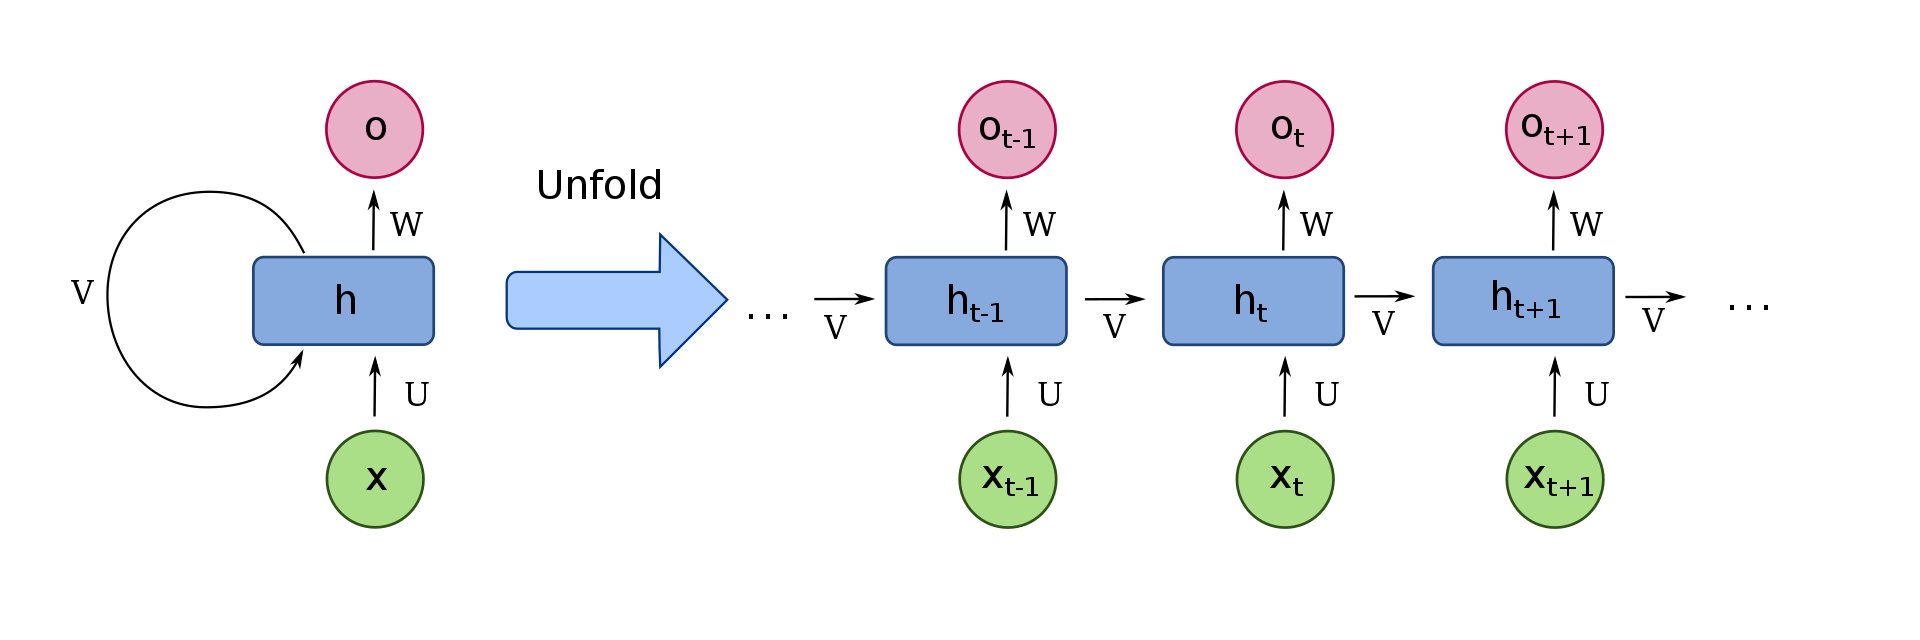
\includegraphics[width=.9\linewidth]{schemat-rnn}
  \caption{Architektura rekurencyjnej sieci neuronowej. Źródło: \cite{WikipediaEN:RNN}}
  \label{fig:schemat-rnn}
\end{figure}
\noindent Rekurencyjna sieć neuronowa była jednym z pierwszych i najpopularniejszych rozwiązań wykorzystywanych przy przetwarzaniu języka naturalnego. Przy jej pomocy można rozwiązać skutecznie wiele zadań, jednakże nie jest wolna od wad. Największym problemem z nią związanym jest duża niestabilność objawiająca się poprzez eksplozję lub zanikanie gradientu. Spowodowane jest to tym, iż w obliczeniach sieci rekurencyjnej za każdym razem uwzględniane są wyniki z poprzedniego przetworzenia. W przypadku chęci przetwarzania długich tekstów, mnożenie kolejnych wartości gwałtownie zwiększa lub zmniejsza wartość gradientu, co znacząco zaburza ostateczny wynik (przykładowo wartość 1,01 podniesiona do tysięcznej potęgi daje wynik ponad 10 tysięcy). W celu zaadresowania tychże problemów powstały rozszerzenia sieci rekurencyjnej. Najpopularniejsze z nich to: Long Short-term Memory \cite{lstm} oraz Gated Reccurent Unit \cite{gru}. Dzięki skomplikowaniu obliczeń oraz przekazywania danych w postaci kontekstu do kolejnych elementów szeregu, zjawisko eksplozji lub zanikania gradientu nie ma aż tak znaczącego wpływu na ostateczne rezultaty, ale mimo to nie jest ono całkowicie wyeliminowane.
% TODO dokładniej opisać co takiego dodały lstm i gru
\subsection{Atencja}
Atencja to kluczowy mechanizm w dziedzinie sieci neuronowych, który pierwszy raz został zaproponowany w 2014 roku \cite{attention}, w celu poprawy działania modelu przetwarzania języka naturalnego skupiającego się na tłumaczeniu tekstu na różne języki. Mechanizm ten został zaproponowany, w celu usprawnienia danych kontekstowych, jakie każdy z elementów przetwarzanej sekwencji posiadał. Idea atencji opiera się na tym, że każda część danych wejściowych może mieć różne znaczenie dla wyniku. Zamiast traktować całą sekwencję jako jedną całość, atencja pozwala modelowi skupić się na istotnych fragmentach danych wejściowych w zależności od kontekstu. W praktyce atencja jest zazwyczaj implementowana jako dodatkowy moduł w sieci neuronowej. Moduł ten oblicza wagi dla poszczególnych części danych wejściowych, które określają, jak bardzo te części powinny być brane pod uwagę przy generowaniu wyniku. Wagi te są obliczane na podstawie podobieństwa między danymi wejściowymi a aktualnym stanem modelu.

Szczególną odmianą mechanizmu atencji jest tak zwana atencja własna, która została zaproponowana po raz pierwszy przez autorów architektury Transformera \cite{transformer}, który okazał się rewolucyjnym rozwiązaniem w dziedzinie przetwarzania języka naturalnego, w głównej mierze dzięki zastosowaniu właśnie atencji własnej. Głównym aspektem odróżniającym ją od klasycznej wersji jest fakt, iż wagi konkretnych elementów obliczane są indywidualnie, biorąc pod uwagę wartości wszystkich pozostałych parametrów, jak i jego samego, skąd pochodzi nazwa samoistnej atencji. Pozwala to na uwzględnienie jedynie istotnych wartości w kontekście konkretnego elementu, a nie tak jak w przypadku klasycznego podejścia, jedynie w kontekście globalnym. Znacząco usprawnia to działanie modelu przetwarzającego teksty zawierające wiele elementów. Dodatkowym usprawnieniem często wykorzystywanym wraz z atencją własną jest mechanizm wielogłowej atencji. Polega on na równoległym wykorzystaniu kilku modułów atencji, a następnie połączeniu ich wyników w ostateczny rezultat. Takie podejście posiada wiele zalet, którymi są między innymi:
\begin{itemize}
  \item wychwytywanie różnorodnych wzorców -- każdy moduł atencji może skupić się na innych aspektach danych wejściowych, co pozwala na wykrycie bardziej złożonych wzorców,
  \item generalizacja -- ze względu na równoległe wykorzystanie wielu modułów, model jest w stanie lepiej radzić sobie z różnorodnością danych wejściowych, co pozwala na osiąganie dobrych wyników w wielu różnorodnych zadaniach.
\end{itemize}
\noindent Mimo tak wielu zalet mechanizm atencji posiada również wiele wad, a są to między innymi:
\begin{itemize}
  \item duża ilość parametrów -- ze względu na konieczność uwzględnienia kontekstu każdego z elementów, moduł atencji musi zaalokować dużą ilość parametrów, co znacząco zwiększa złożoność modelu, a co za tym idzie czas potrzebny na przetworzenie danych, jak i ilość pamięci koniecznej do zaalokowania architektury. W przypadku wykorzystywania wielogłowej atencji problem ten dodatkowo się nasila ze względu na wykorzystywanie równoległych modułów.
  \item Wyniki otrzymane poprzez wykorzystanie modułu atencji mogą być trudne do wyjaśnienia i zinterpretowania -- w przeciwieństwie do tradycyjnych sieci neuronowych, w których znaczenie każdej cechy wejściowej można łatwo określić poprzez sprawdzenie odpowiednich wag, mechanizm uwagi przypisuje znaczenie dynamicznie w czasie działania. Ten dynamiczny charakter utrudnia zapewnienie jasnych wyjaśnień procesu decyzyjnego modelu, utrudniając przejrzystość i interpretowalność.
  \item Duże ilości danych -- ze względu na złożoność mechanizmu oraz dużą ilość parametrów konieczne jest wykorzystanie dużej ilości danych treningowych, aby osiągnąć zadowalające efekty. Istnieją modyfikacje mechanizmu atencji, a w szczególności architektury Transformera \cite{xu2021optimizing}, którym udaje się osiągnąć zadowalające wyniki przy wykorzystaniu mniejszej ilości danych, jednakże są to rozwiązania niestandardowe, które wymagają dodatkowych zabiegów w celu osiągnięcia zadowalających wyników, co pokazuje kolejną wadę wykorzystywania mechanizmu atencji -- złożoność implementacyjną.
\end{itemize}

\subsection{Wizja komputerowa}
Przetwarzanie wszelkiego rodzaju obrazów cyfrowych w postaci zdjęć czy filmów jest niezwykle problematyczne, ponieważ pojedyncze zdjęcie wykonane w jakości HD posiada prawie milion pikseli. Dodatkowo biorąc pod uwagę wiele kombinacji, w których zdjęcie może być wykonane: różne ułożenie przedmiotu, kadr oświetlenie otoczenie, dane konieczne do przetworzenia oraz sformułowanie na ich podstawie algorytmów rozwiązujących dużą część problemów z nimi związanych jest praktycznie niemożliwe. Z tychże względów ogromną popularnością wśród rozwiązywania problemów związanych z wizją komputerową cieszą się algorytmy uczenia maszynowego, a w szczególności splotowe sieci neuronowe. Schemat podstawowej architektury takiej sieci służącej do klasyfikacji obrazu został przedstawiony na rysunku \ref{fig:schemat-cnn}.
\begin{figure}[H]
  \centering
  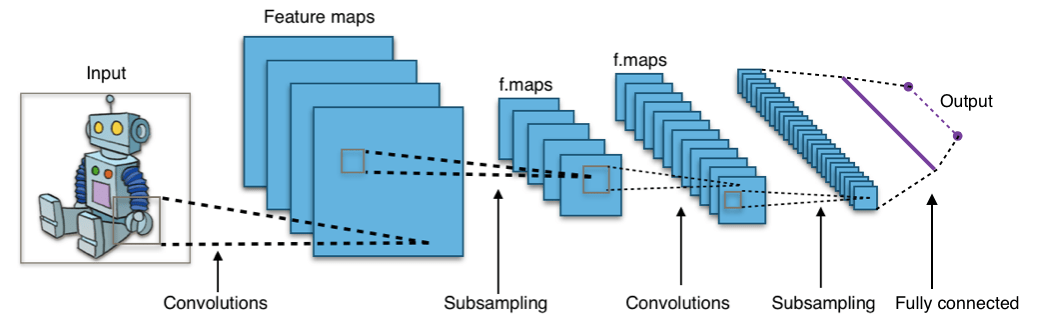
\includegraphics[width=.9\linewidth]{schemat-cnn}
  \caption{Architektura splotowej sieci neuronowej. Źródło: \cite{WikipediaEN:CNN}}
  \label{fig:schemat-cnn}
\end{figure}
\noindent Charakteryzują się one różnymi rodzajami warstw. Do podstawowych typów warstw należą:
\begin{itemize}
  \item warstwa splotowa -- jest to podstawowa warstwa, która składa się z zestawu filtrów splotowych wykorzystujących operację splotu. Filtry te przesuwają się po obrazie wejściowym i wykrywają w nim wzorce o różnym stopniu skomplikowania.
  \item Warstwa aktywacji -- wyniki operacji splotu są przetwarzane za pomocą funkcji aktywacji, takiej jak tangens hiperboliczny, co pozwala na generowanie tak zwanych map cech dla każdego filtra z warstwy splotowej.
  \item Warstwa grupująca -- rozmiar otrzymanych map cech wygenerowanych przez warstwę splotową jest redukowany poprzez grupowanie wartości w oknie i zastępowanie ich pojedynczą wartością reprezentującą cechy w danym obszarze. Najczęściej stosowane są dwa rodzaje operacji grupujących: max-pooling i average-pooling.
\end{itemize}
Powyższe warstwy najczęściej występują wielokrotnie w obrębie jednej sieci, co pozwala na wydobywanie wzorców z przetwarzanego obrazu na różnym poziomie kontekstu. Dalsze przetwarzanie oraz grupowanie map cech obrazu daje możliwość uwzględnienia szerszego kontekstu, jaki jest zawarty w obrazie niż jedynie w obrębie najbliższego sąsiedztwa danego piksela.
\subsection{Mechanizm atencji w przetwarzaniu obrazów}
% TODO Opisać jak działa atencja w dziedzinie wizji komputerowej
\subsection{Wstępne przetwarzanie danych}
W procesie przygotowywania danych do przetwarzania przez sieci neuronowe konieczne jest dokładne ujednolicenie i przekształcenie danych w formę, która jest łatwo przyswajalna przez komputer. Dla obrazów cyfrowych, które są reprezentowane jako macierze kodów RGB, wystarcza zazwyczaj znormalizowanie wartości pikseli oraz ujednolicenie ich wymiarów w celu ułatwienia obliczeń. W przypadku danych o niestandardowym formacie pojawia się dodatkowy krok, jakim jest konwersja obrazów do formatu RGB.
Częstą dodatkową techniką, która pozwala na zwalczanie problemów przetrenowania oraz małej ilości danych treningowych jest przycinanie obrazów.
Stosuje się do tego kilka technik:
\begin{itemize}
  \item przycinanie losowe,
  \item przycinanie z wykorzystaniem algorytmów wykrywania krawędzi.
\end{itemize}
\noindent Wybór odpowiedniej techniki w głównej mierze jest zależny od potrzeb wynikających z docelowego problemu, który ma zostać rozwiązany poprzez wykorzystanie sieci neuronowej. Przy pomocy tejże techniki możliwe jest również wielokrotne wykorzystanie tego samego zdjęcia jako zupełnie innego obrazu, ze względu na przycięcie i zawarcie na nim innych elementów, co znacząco zwiększa ilość dostępnych danych treningowych.

W przypadku wartości tekstowych, które są wartością wejściową całej architektury, proces przetwarzania jest bardziej skomplikowany. Tekst w języku naturalnym posiada różnorodność, obejmującą zmienność długości słów, różne końcówki, a także inne nieregularności. Aby uporządkować te rozbieżności, stosuje się kilka technik:
\begin{itemize}
  \item normalizacja wielkości liter -- wszystkie litery w tekście są zamieniane na małe litery.
  \item Usunięcie wszystkich znaków niebędących słowami takich jak kropki, przecinki, emotikony.
  \item Usunięcie słów znajdujących się na stop liście, czyli zbiorze słów o nikłym znaczeniu dla kontekstu zdania, takich jak spójniki, przyimki lub nawet często używane słowa.
  \item W przypadku chęci osiągnięcia znaczącej generalizacji często stosowane jest również odrzucenie rzadko występujących słów w celu zmniejszenia dostępnego słownika, a co za tym idzie, zwiększenia skuteczności uczenia.
\end{itemize}
\noindent Tak przetworzony tekst nadal jest w postaci słów i liter, co jest problematycznym formatem przetwarzania dla komputera -- porządanymi danymi są macierze i wektory, którymi operują wszelkie algorytmy uczenia maszynowego. W celu osiągnięcia takowego formatu, stosuje się technikę zwaną tokenizacją, z której można wyodrębnić kilka różnych podejść. Do najpopularniejszych należą:
\begin{itemize}
  \item tokenizacja znaków -- jest najprostszą techniką polegającą na utworzeniu wektorów, gdzie pojedynczą wartością jest każdy znak przetwarzanego zdania. Takie podejście znacząco zwiększa ilość przetwarzanych danych, co nie jest konieczne, ponieważ pojedyncze litery ze słów nie nie niosą ze sobą znaczących informacji -- informacja zawarta jest w całości słowa, a nawet w kontekście kilku słów lub całego zdania. Dużym atutem tego podejścia jest brak konieczności stosowania pozostałych technik wstępnego przetwarzania tekstu, co znacząco upraszcza proces.
  \item tokenizacja słów -- polega na wyodrębnieniu token na podstawie słów. To właśnie do tej techniki najczęściej stosowane są wcześniej wspomniane metody wstępnego przetwarzania tekstu. W odróżnieniu od tokenizacji znaków, gdzie liczba liter w słowniku jest znacząco ograniczona, ilość słów może osiągać ogromne wartości -- Wielki słownik ortograficzny PWN zawiera 140 tysięcy haseł \cite{pwn2016}, dlatego konieczne jest zastosowanie pewnych ograniczeń tak jak wspomniane wcześniej odrzucanie rzadko występujących słów.
  \item tokenizacja digramowa -- polega na znalezieniu par liter i traktowaniu ich jako pojedynczy token. Wykorzystanie tejże techniki pozwala na uwzględnienie o wiele szerszego kontekstu niż w podstawowej tokenizacji znaków jednocześnie nie ograniczając się do konkretnego słownika słów, co umożliwia generowanie danych spoza słownika.
\end{itemize}
\noindent W przetwarzaniu języka dodatkową trudność wprowadza fakt, iż nie istnieje jeden uniwersalny język, a wiele popularnych języków posiada swoje własne specyficzne cechy, jak na przykład zupełnie inny alfabet, czy brak spacji między słowami. Rozwiązaniem tego problemu może być próba rozpoznania języka, a następnie zastosowanie odrębnej techniki przetwarzania dla konkretnej rodziny językowej.
